\documentclass[a4paper,UTF8]{article}
\usepackage{ctex}
\usepackage[margin=1.25in]{geometry}
\usepackage{color}
\usepackage{graphicx}
\usepackage{amssymb}
\usepackage{amsmath}
\usepackage{amsthm}
\usepackage{enumerate}
\usepackage{bm}
\usepackage{hyperref}
\usepackage{pgfplots}
\usepackage{epsfig}
\usepackage{color}
\usepackage{tcolorbox}
\usepackage{mdframed}
\usepackage{lipsum}
\usepackage{natbib}
\usepackage{pythonhighlight}
\newmdtheoremenv{thm-box}{myThm}
\newmdtheoremenv{prop-box}{Proposition}
\newmdtheoremenv{def-box}{定义}

\setlength{\evensidemargin}{.25in}
\setlength{\textwidth}{6in}
\setlength{\topmargin}{-0.5in}
\setlength{\topmargin}{-0.5in}
% \setlength{\textheight}{9.5in}
%%%%%%%%%%%%%%%%%%此处用于设置页眉页脚%%%%%%%%%%%%%%%%%%
\usepackage{fancyhdr}                                
\usepackage{lastpage}                                   
\usepackage{layout}                                     
\newtheorem*{solution}{Solution}

\footskip = 10pt 
\pagestyle{fancy}                    % 设置页眉                 
\lhead{2020年秋季}                    
\chead{高级机器学习}                                                
% \rhead{第\thepage/\pageref{LastPage}页} 
\rhead{作业二}                                                                                               
\cfoot{\thepage}                                                
\renewcommand{\headrulewidth}{1pt}  			%页眉线宽,设为0可以去页眉线
\setlength{\skip\footins}{0.5cm}    			%脚注与正文的距离           
\renewcommand{\footrulewidth}{0pt}  			%页脚线宽,设为0可以去页脚线

\makeatletter 									%设置双线页眉                                        
\def\headrule{{\if@fancyplain\let\headrulewidth\plainheadrulewidth\fi%
\hrule\@height 1.0pt \@width\headwidth\vskip1pt	%上面线为1pt粗  
\hrule\@height 0.5pt\@width\headwidth  			%下面0.5pt粗            
\vskip-2\headrulewidth\vskip-1pt}      			%两条线的距离1pt        
 \vspace{6mm}}     								%双线与下面正文之间的垂直间距              
\makeatother  

%%%%%%%%%%%%%%%%%%%%%%%%%%%%%%%%%%%%%%%%%%%%%%
\numberwithin{equation}{section}
%\usepackage[thmmarks, amsmath, thref]{ntheorem}
\newtheorem{myThm}{myThm}
\newtheorem*{myDef}{Definition}
\newtheorem*{mySol}{Solution}
\newtheorem*{myProof}{Proof}
\newtheorem*{myRemark}{备注}
\renewcommand{\tilde}{\widetilde}
\renewcommand{\hat}{\widehat}
\newcommand{\indep}{\rotatebox[origin=c]{90}{$\models$}}
\newcommand*\diff{\mathop{}\!\mathrm{d}}

\usepackage{multirow}

%--

%--
\begin{document}
\title{高级机器学习\\
大作业}
\author{俞星凯\, 171830635} 
\maketitle
%%%%%%%% 注意: 使用XeLatex 编译可能会报错,请使用 pdfLaTex 编译 %%%%%%%

\section*{学术诚信}

本课程非常重视学术诚信规范,助教老师和助教同学将不遗余力地维护作业中的学术诚信规范的建立。希望所有选课学生能够对此予以重视。\footnote{参考尹一通老师\href{http://tcs.nju.edu.cn/wiki/}{高级算法课程}中对学术诚信的说明。}

\begin{tcolorbox}
	\begin{enumerate}
		\item[(1)] 允许同学之间的相互讨论,但是{\color{red}\textbf{署你名字的工作必须由你完成}},不允许直接照搬任何已有的材料,必须独立完成作业的书写过程;
		\item[(2)] 在完成作业过程中,对他人工作(出版物、互联网资料)中文本的直接照搬(包括原文的直接复制粘贴及语句的简单修改等)都将视为剽窃,剽窃者成绩将被取消。{\color{red}\textbf{对于完成作业中有关键作用的公开资料,应予以明显引用}};
		\item[(3)] 如果发现作业之间高度相似将被判定为互相抄袭行为,{\color{red}\textbf{抄袭和被抄袭双方的成绩都将被取消}}。因此请主动防止自己的作业被他人抄袭。
	\end{enumerate}
\end{tcolorbox}

\section*{作业提交注意事项}
\begin{tcolorbox}
	\begin{enumerate}
		\item[(1)] 请在LaTeX模板中{\color{red}\textbf{第一页填写个人的姓名、学号信息}};
		\item[(2)] 本次作业需提交该pdf文件、直接可以运行的源码,将以上几个文件压缩成zip文件后上传。zip文件格式为{\color{red}\textbf{学号.zip}},例如170000001.zip;pdf文件格式为{\color{red}\textbf{学号\_姓名.pdf}},例如170000001\_张三.pdf。
		\item[(3)] 未按照要求提交作业,或提交作业格式不正确,将会{\color{red}\textbf{被扣除部分作业分数}};
		\item[(4)] 本次作业提交截止时间为{\color{red}\textbf{1月8日23:59:59}}。除非有特殊情况(如因病缓交),否则截止时间后不接收作业,本次作业记零分。
	\end{enumerate}
\end{tcolorbox}

\newpage
\section{Introduction}
本次的作业为使用条件随机场(conditional random field,CRF)解决OCR(optical character recognition)问题。

在CRF模型中,有两种变量:我们要建模的隐藏变量和始终观察到的变量。对于OCR,我们要在观察的字符图像(也就是每个图像对应的像素数组)的情况下,对字符(例如“a”或“c”)进行建模。通常来说,未观察到的变量用$Y$表示,观察到的变量用$X$表示。CRF试图对$P(Y|X)$建模,即给定观察到的图像上字符的条件分布。该模型的结构如\ref{Fig.main1}下所示:
\begin{figure}[h] 
\centering
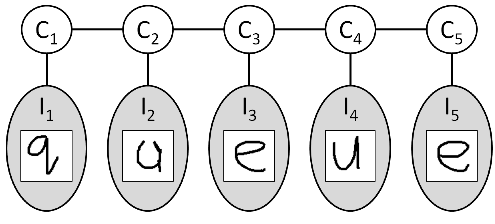
\includegraphics[width=0.7\textwidth]{figs/fig1.png} 
\caption{Markov Network} 
\label{Fig.main1}
\end{figure}

在CRF中,每个特征都对应一个权重$\theta_i$,在给定特征和权重的情况下,条件概率分布可以表示为:
\begin{equation}
P(\mathbf{Y} \mid \mathbf{x}: \theta)=\frac{1}{Z_{\mathbf{x}}(\theta)} \exp \left\{\sum_{i=1}^{k} \theta_{i} f_{i}\left(\mathbf{Y}, \mathbf{x}\right)\right\}\label{eq1}
\end{equation}

其中,$Z_x(\theta)$为配方函数
\begin{equation}
Z_{\mathbf{x}}(\theta) \equiv \sum_{\mathbf{Y}} \exp \left\{\sum_{i=1}^{k} \theta_{i} f_{i}\left(\mathbf{Y}, \mathbf{x}\right)\right\}
\end{equation}

在这次的任务中,一共有三类特征,三类特征均为指示函数,即满足条件时$f=1$,不满足时$f=0$:
\begin{itemize}
    \item $f_{i, c}^{C}\left(Y_{i}\right)$,指示是否$Y_i = c$
    \item $f_{i, j, c, d}^{I}\left(Y_{i}, x_{i j}\right)$,指示是否$Y_i=c,x_{ij}=d$
    \item $f_{i, c, d}^{P}\left(Y_{i}, Y_{i+1}\right)$,指示是否$Y_i=c,Y_{i+1}=d$
\end{itemize}

建立好模型,给定训练样本,我们就可以使用最大似然估计来进行学习:
\begin{equation}
    LL(\mathbf{x},\mathbf{Y},\theta) =\sum_{i=1}^{k} \theta_{i} f_{i}(\mathbf{Y}, \mathbf{x}) -\log \left(Z_{\mathbf{x}}(\theta)\right)\label{eq2}
\end{equation}

对于这个目标,我们可以使用梯度上升算法学习参数。

\section{Dataset}
本题中的数据集一共包含两个部分\texttt{trainset}和\texttt{testset}, 分别是训练集和测试集.训练集中有400个样本,测试集中有200个样本. 每个样本被存储在一个\texttt{txt}文件中, 第一行为对应的单词, 之后的每行为单词的每个字母对应的像素的状态.

\section{Assignment}
\begin{enumerate}
    \item 建立CRF模型,在训练集上进行训练,使用梯度上升的方法对模型参数进行求解,即求解公式\eqref{eq2}(注:不允许使用现有的CRF包,使用python实现)。
    \item 在模型训练完成后,在测试集上进行推断,评价模型的性能。
    \item 使用一些其他方法提高模型性能,可参考以下几个方面但不限于此:
    \begin{itemize}
        \item 提高模型表达能力:如在CRF图上添加新的连接。
        \item 缓解模型过拟合:如添加正则项。
        \item 加速模型训练过程:如权重共享。
    \end{itemize}
    \item 完成实验报告,主要包含具体的实现方法,如何复现运行代码,对模型的改进以及结果的分析等部分。
\end{enumerate}
\section {实验报告}
~\\
本次实验完全自主实现链式条件随机场,没有参考任何现成代码。\\
非常感谢(李航,统计学习方法,2019)的第11章对条件随机场深入浅出的介绍,没有它我不可能完成本次实验。\\
代码尽最大可能向量化计算,使得训练非常快速,能够在1分钟内对所有400个训练数据完成500轮参数迭代,并且效果非常好。在测试集上,字符准确率高达88\%(对应位置字符匹配),全词准确率53.5\%(整个单词完全匹配),在训练集上,字符准确率89\%,全词准确率53.8\%。可以看到模型的训练集性能仅比测试集性能略高一点,没有出现过拟合。\\
模型中有三类特征函数,相应地有三类参数,代码中使用$theta_1$、$theta_2$、$theta_3$表示。26代表26个英文字母,注意$theta_2$中,因为每个字符对应321个01比特,所以用321*2=642表示,前321个对应第二类指示$Y_i=c,x_{ij}=0$的特征函数,后321个对应第二类指示$Y_i=c,x_{ij}=1$的特征函数。
\begin{python}
theta1 = np.ones(26) * 0.1
theta2 = np.ones((26, 642)) * 0.1
theta3 = np.ones((26, 26)) * 0.1
\end{python}
数据预处理比较简单,不作赘述。读取数据之后,我们构造三类特征函数。
\begin{python}
trainX, trainY = Load('Dataset/train')
m = len(trainY)
f1 = np.zeros((m, 14, 26), np.bool)
f2 = np.zeros((m, 14, 26, 642), np.bool)
f3 = np.zeros((m, 14, 26, 26), np.bool)
for k in range(m):
    feature, label = trainX[k], trainY[k]
    for i, c in enumerate(label):
        f1[k, i, c] = 1
        f2[k, i, c, :321] = 1 - feature[i]
        f2[k, i, c, 321:] = feature[i]
    for i in range(len(label)-1):
        f3[k, i, label[i], label[i + 1]] = 1
\end{python}
因为$\theta$是位置无关的,同一特征在各个位置都有定义,可以对同一特征在各个位置求和,将“局部”特征函数转化为“全局特征函数”(李航,统计学习方法,2019,221-222)。
\begin{python}
g1 = f1.sum(axis=1)
g2 = f2.sum(axis=1)
g3 = f3.sum(axis=1)
\end{python}
任务难点主要在于梯度计算,公式\eqref{eq2}中对数似然分为两部分,我们针对两部分分别求梯度。\\
第一部分的梯度比较简单,容易看出参数$theta_i$在第$k$个样本上的第一部分梯度正是$g_i[k]$,$i=1,2,3$。\\
第二部分的梯度比较困难,基于(李航,统计学习方法,2019,223)给出的条件随机场矩阵形式,使用下面代码计算所有矩阵$Ms$和规范化因子$Z$。
\begin{python}
size = len(feature)
Ms = np.zeros((size, 26, 26))
Z = np.exp(theta1 + theta2 @ feature[0])
Ms[0, 0] = Z
for i in range(1, size):
    W = theta1 + theta2 @ feature[i] + theta3
    M = np.exp(W)
    Z = Z @ M
    Ms[i] = M
Z = Z @ np.ones(26)
\end{python}
对第二部分的梯度进行公式推导,结果是
\[\frac{\partial\log\left(Z_{\mathbf{x}}(\theta)\right)}{\partial\theta_i} = \frac{\sum_{\mathbf{Y}} \exp \left\{\sum_{i=1}^{k} \theta_{i} f_{i}\left(\mathbf{Y}, \mathbf{x}\right)\right\}f_{i}\left(\mathbf{Y}, \mathbf{x}\right)}{Z_{\mathbf{x}}(\theta)}\]
我们可以将分子看作仅对满足$f\left(\mathbf{Y}, \mathbf{x}\right)=1$的$\mathbf{Y}$求和,忽略不满足条件的$\mathbf{Y}$。\\
为了减少冗余计算,使用前向后向算法(李航,统计学习方法,2019,225),计算$alpha$和$beta$,其中$alpha[i, j]$表示在位置$i$的标记是$j$并且从$0$到$i$的非规范化概率,$beta[i, j]$表示在位置$i$的标记是$j$并且从$i+1$到$n$的非规范化概率。
\begin{python}
alphas = np.zeros((size, 26))
alphas[0] = Ms[0, 0]
for i in range(1, size):
    alphas[i] = alphas[i - 1] @ Ms[i]
betas = np.zeros((size, 26))
betas[size - 1] = np.ones(26)
for i in range(size - 2, -1, -1):
    betas[i] = Ms[i + 1] @ betas[i + 1]
\end{python}
满足第一类特征条件$f\left(\mathbf{Y}, \mathbf{x}\right)=\mathbb{I}(\mathbf{Y}_i=j)$的非规范化概率正是$alpha[i, j] * beta[i, j]$,将其向量化,得到$theta_1$的第二部分梯度$delta_1$。
\begin{python}
delta1 = np.sum(alphas * betas, axis=0) / Z
\end{python}
满足第二类特征条件的样本,对应的参数是$theta_2$中$feature[i]$为1的那些列,这些列上的梯度都是$delta_1$。
\begin{python}
delta2 = np.zeros((26, 642))
for i in range(len(feature)):
    # delta2[:, feature[i]] += delta1
    delta2 += np.outer(delta1, feature[i])
\end{python}
满足第三类特征条件$f\left(\mathbf{Y}, \mathbf{x}\right)=\mathbb{I}(\mathbf{Y}_{i-1}=j\land\mathbf{Y}_i=k)$的非规范化概率是$alpha[i-1, j] * Ms[i, j, k] * beta[i, k]$,向量化得到$delta_3$。
\begin{python}
delta3 = np.zeros((26, 26))
for i in range(1, l):
    delta3 -= Ms[i] * np.outer(alphas[i - 1], betas[i]) / Z
\end{python}
训练部分至此完毕,每轮使用前向后向算法计算$alpha$和$beta$,然后计算梯度$delta_1$、$delta_2$和$delta_3$,最后使用梯度上升更新参数。注意以上描述都是针对一个样本的,实际代码中每轮计算了训练集所有样本的梯度并取平均,用以更新参数。\\
测试部分比较简单,针对每个样本计算$alpha$和$beta$,矩阵$alpha*beta$的第$i$行第$j$列表示第$i$个位置是第$j$个字符的非规范化概率,我们取最大的预测即可。
\end{document}